 \label{desenvolvimento_eletromecanica}

Nesta seção é descrito o detalhamento da solução e finalização do módulo de eletromecânica, bem como mudanças que ocorreram e a descrição da integração final com todos os sub-módulos resultando na entrega do produto final previsto na Fase 04.

\subsection{Detalhamento do Módulo}

%%%%%%%%%% SUMARIZAR TODO O TRABALHO QUE FOI FEITO ATÉ AGORA PARA ENTREGA O SUBMÓDULO %%%%%%%%%%%%%%

\subsection{Detalhamento da Integração Final}

%%%%%%%%%% REALIZAR DETALHAMENTO DO TRABALHO DE INTEGRAÇÃO FINAL %%%%%%%%%%%%%%%

% Nesta seção é descrito o detalhamento da solução do módulo de eletromecânica, resultante das duas primeiras fases,
% e o seu projeto e construção, resultante da Fase 03.

% \subsection{Detalhamento da Solução}

% O detalhamento da solução para a frente de eletromecânica pode ser sumarizado nos itens abaixo. A solução completa definida nas
%   Fases 01 e 02 pode ser vista no \href{https://drive.google.com/file/d/0B5InkGKx6O-MR1B3eVYzZFpjQ3c/view?usp=sharing}{Relatório 1}.

% Para a construção de uma bancada com capacidade de vibração mecânica e análise de parâmetros, é de interesse um sistema de estudos para comportamento mecânico frente às vibrações, sendo um equipamento para instalações fixas com limites de carga e dimensões para sistemas analisados. Portanto, para análise eletromecâmica, seguem os estudos realizados abaixo.

% \begin{figure}[h!]
% 	\centering
% 		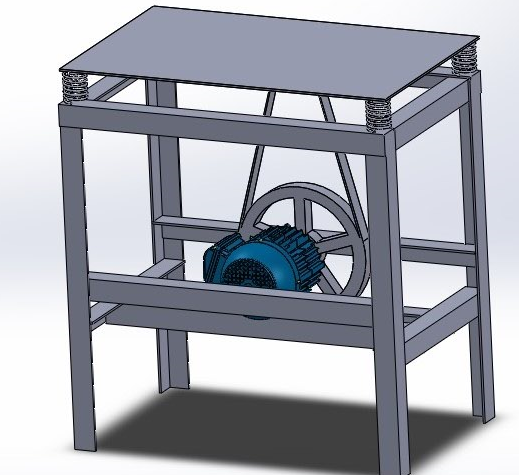
\includegraphics[keepaspectratio=true,scale=0.6]{figuras/1.png}
% 	\caption{Bancada para ensaio de teste de vibração mecânica. Fonte: Autores}
%     \label{bancada}
% \end{figure}

% As funções principais do controle de um motor são: partida, parada, direção de rotação, regulação da velocidade, limitação da corrente de partida, proteção mecânica e proteção elétrica. Um motor só começa a girar quando o momento de carga a ser vencido, quando parado, for menor do que seu conjugado de partida. Em determinadas aplicações há necessidade de uma rápida desaceleração do motor e da carga.

% \begin{figure}[h!]
% 	\centering
% 		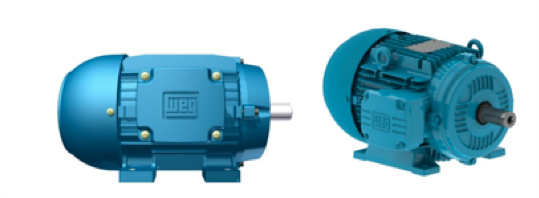
\includegraphics[keepaspectratio=true,scale=0.6]{figuras/2.png}
% 	\caption{- Motor de indução trifásica. Fonte: \cite{WEG}}
%     \label{motor}
% \end{figure}

% O modo utilizado para variação de velocidade do motor de indução será através do inversor de frequência, o qual possibilita o controle do motor
% CA variando a frequência, mas também realiza a variação da tensão de saída para que seja respeitada a característica V/F ( Tensão / Freqüência) do motor.

% \subsection{Projeto e Construção}

% No projeto em questão, será usado um motor de indução trifásico conectado a um eixo preso por mancais soldados no tampo da mesa,
% usando-se para isto uma correia encaixada na polia fixa no eixo do motor e no eixo preso nos rolamentos dos mancais.
% Com isso, tem-se o intuito de acionar o sistema, gerando assim uma vibração. Para realizar esta vibração, a velocidade do motor será
% alterada com o uso de um inversor de frequência e com a razão de voltas da polia fixa no motor e o do eixo fixo nos mancais.
% O conjunto motor e inversor dimensionado deverá atender o torque solicitado e as velocidades solicitadas por todo o sistema.

% 	Para avaliação térmica do motor realizado por meio da tecnologia do termovisor, na qual fornece uma avaliação da temperatura para com a classe de isolamento, na qual podemos observar na figura \ref{camera} abaixo o comportamento térmico do mesmo para a classe de isolamento do tipo F.

% \begin{figure}[h!]
%     \centering
% 	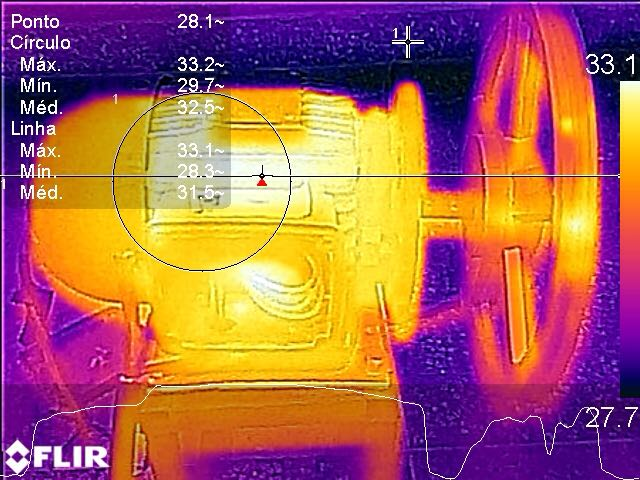
\includegraphics[keepaspectratio=true,scale= 0.5]{figuras/camera.jpg}
% 	\caption{- Câmara térmica. Fonte: Autores}
%     \label{camera}
% \end{figure}

% No projeto em questão optamos pela ligação do motor em estrela, dada que a disponibilidade da rede elétrica local é 380 V.

% \begin{figure}[!h]
% 	\centering
% 		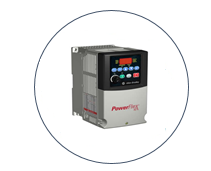
\includegraphics[keepaspectratio=true,scale=1.0]{figuras/3.png}
% 	\caption{Inversor de frequência elegido. Fonte: \cite{allen}}
%     \label{inversor}
% \end{figure}

% O inversor de frequência trabalha com rampas para partida e frenagem. Na partida é utilizada a rampa de aceleração, a velocidade inicia em zero e atinge a velocidade desejada, podendo ajudar o tempo numa faixa de milésimos de segundo. A frequência do rotor é maior do que a frequência do estator durante a frenagem, dessa forma é provocado um fluxo reverso da energia do rotor diretamente ao estator (COVINO; GRASSI; PAGANO, 1997). A rampa de desaceleração é responsável por controlar a frenagem, esse processo se dá pela redução de forma controlada da frequência aplicada ao motor.
% A Figura \ref{rampas} abaixo evidencia as rampas de aceleração e desaceleração.

% \begin{figure}[h!]
% 	\centering
% 		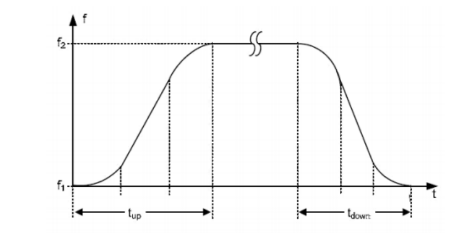
\includegraphics[keepaspectratio=true,scale=0.9]{figuras/4.png}
% 	\caption{Rampas de aceleração e desaceleração geradas pelo inversor de frequência. \cite{siemens}}
%     \label{rampas}
% \end{figure}

% \subsubsection*{Medidas construtivas}

% Na primeira parte do trabalho, basicamente realizou-se um estudo sobre o tema proposto, definiu-se os conceitos básicos, realizou-se os cálculos iniciais para definição das diretrizes a serem tomadas e definiu-se qual o motor e o inversor a ser usado. Após a realização do ponto de controle 1, foram tomadas as seguintes medidas construtivas:

% \begin{itemize}
% \item Aquisição do motor de indução trifásico de 0,5 cv;
% \item Aquisição do inversor de frequência da marca Bradley;
% \item Aquisição de cabos trifásicos de 2,5cm de diâmetros, valor calculado de acordo com a norma 5410;
% \item Aquisição de tomadas trifásicas com capacidade de 10 A;
% \item Realização do cabeamento do motor, sendo este ligado em estrela de acordo com o indicado em sua placa de identificação;
% \item Realização do cabeamento do inversor de frequência, sendo um cabeamento para ligação na fonte de alimentação e o outro para conexão com o motor de indução;
% \item Realização de testes no motor, verificando que o mesmo encontra-se em perfeitas condições de funcionamento;
% \item Realização de medição da corrente em cada fase do motor;
% \item Realização de teste de temperatura no motor de indução, com o auxílio de uma câmera térmica;
% \item Estudo do inversor de frequência para conhecimento de seus parâmetros de funcionamento;
% \item Parametrização do inversor afim de satisfazer a necessidade do projeto;
% \item Realização de testes de partida e frenagem do motor, usando-se o inversor de frequência;
% \item Fixação do motor de indução na estrutura da bancada;
% \item Definição do sistema de proteção.
% \end{itemize}


% A tabela \ref{tabela_info_motor} mostra os dados elétricos do motor de indução escolhido.

%         \begin{table}[h]
%             \begin{center}
%               \begin{tabular}{|p{5cm}|p{5cm}|}
%                 \hline
%                 \textbf{Dados elétrico do motor} &
%                 \\ \hline
%                 Carcaça & 71
%                 \\ \hline
%                 Potência & 0,5HP
%                 \\ \hline
%                 Frequencia & 60Hz
%                 \\ \hline
%                 Polos & 4
%                 \\ \hline
%                 Rotação Nominal & 1720 RPM
%                 \\ \hline
%                 Escorregamento & 4,44
%                 \\ \hline
%                 Tensão Nominal & 220/380 V
%                 \\ \hline
%                 Corrente Nominal & 2.07/1.20 A
%                 \\ \hline
%                 Corrente de Partida & 10.45/5.99 A
%                 \\ \hline
%                 LP/LN & 5.0
%                 \\ \hline
%                 Corrente a vazio & 1.50/0.868 A
%                 \\ \hline
%                 Conjugado Nominal & 2.06 Nm
%                 \\ \hline
%                 Conjugado de partida & 240
%                 \\ \hline
%                 Conjugado Máximo & 250
%                 \\ \hline
%                 Categoria & N
%                 \\ \hline
%                 Classe de isolação & B
%                 \\ \hline
%                 Elevação de temperatura & 80 K
%                 \\ \hline
%                 Tempo de rotor bloqueado & 18 s (quente)
%                 \\ \hline
%                 Fator de serviço & 1.15
%                 \\ \hline
%                 Regime de serviço & S1
%                 \\ \hline
%                 Temperatura ambiente & -20 graus Celsius - +40 graus Celsius
%                 \\ \hline
%                 Altitude & 1000 m
%                 \\ \hline
%                 Proteção & IP55
%                 \\ \hline
%                 Massa aproximada & 10 Kg
%                 \\ \hline
%                 Momento de inércia & 0,00082 Kg
%                 \\ \hline
%                 Nível de ruído & 47 dB(A)
%                 \\ \hline
%               \end{tabular}
%               \caption[Informações detalhadas sobre o motor]{Informações detalhadas sobre o motor
%               \protect Fonte: \cite{WEG_catalogo}}
%             \label{tabela_info_motor}
%         \end{center}
%     \end{table}


% \subsubsection*{Parametrização do inversor de frequência}

% Após a realização do estudo acerca do inversor de frequência, foi realizada a parametrização do mesmo. Com base no manual disponibilizado pela NHP \textit{Eletrical Engineering Products}, uma empresa australiana renomada no setor da engenharia elétrica, o controle do motor foi minimamente estabelecido em todos os detalhes necessários para atender a demanda do projeto.

% O inversor dispõe de uma interface bastante amigável, como pode ser visto na Figura \ref{Interface do inversor}

% \begin{figure}[h!]
% 	\centering
% 		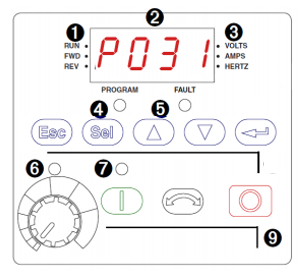
\includegraphics[keepaspectratio=true,scale=0.6]{figuras/interface_inversor.png}
% 	\caption{Interface do inversor de frequência. Fonte: NHP}
%     \label{Interface do inversor}
% \end{figure}

% Para a programação do inversor, foi utilizado apenas os parâmetros básicos, visto que, dessa forma, a nossa necessidade seria atendida. A Figura \ref{Parâmetros do inversor} mostra os parâmetros utilizados para fazer o controle do motor de indução através do inversor de frequência.

% \begin{figure}[h!]
% 	\centering
% 		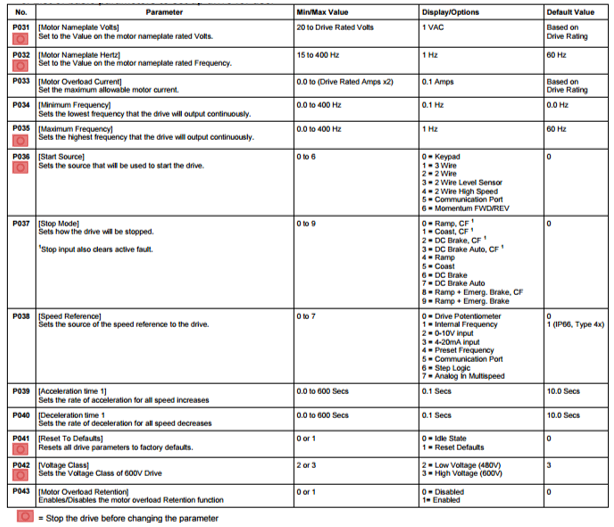
\includegraphics[keepaspectratio=true,scale=0.9]{figuras/parametros_inversor.png}
% 	\caption{Listagem dos parâmetros básicos utilizados. Fonte: NHP}
%     \label{Parâmetros do inversor}
% \end{figure}

% No parâmetro P031 foi ajustada a tensão na qual o motor necessita, no caso a tensão foi ajustada em 380V. No parâmetro P032 foi ajustada a frequência nominal do motor de indução, fixada em 60Hz. O parâmetro P033 não foi alterado. Os parâmetros P034 e P035 remetem, respectivamente, às frequências mínima e máxima, ajustadas em 0 e 60Hz. O parâmetro P036 estabelece de que forma o start ocorrerá, no caso foi selecionada a opção 0 que estabelece que será pelo botão na interface do inversor de frequência. O parâmetro P037 não foi alterado. Já o parâmetro P038 foi ajustado na opção 2, cuja estabelece o controle via entrada de 0 a 10V, nessa parte acontece a integração com a frente de eletroeletrônica, onde haverá o controle estabelecido por eles. Os parâmetros P039 e P040 estabelecem os tempos de aceleração e desaceleração, respectivamente, esses tempos estão definidos em valores por volta de 2 a 4 segundos. Os últimos três parâmetros não foram alterados.

% \subsubsection*{Sistema de Segurança}

% Sistemas de segurança elétrica são concebidos com a finalidade de garantir uma operação segura para os usuários finais, equipes de manutenção e dos próprios equipamentos, que em casos de ocorrências internas ou externas os danos são minimizados.

% O projeto inicial concebia a utilização além dos disjuntores e fusíveis, a utilização de dispositivos anti-surto, no sistema trifásico bem como um diferencial residual, no entanto para fins de minimização de custos, considerando a fase de protótipo, foram considerados apenas a utilização de fusíveis na entrada principal trifásica e disjuntores com função de desarme e dispositivo do manobra nos diferentes circuitos que são: Inversor-motor, controle eletrônico, e tomadas auxiliares, dispostos segundo o diagrama mostrado na Figura \ref{Diagrama de Instalações}.

% \begin{figure}[h!]
% 	\centering
% 		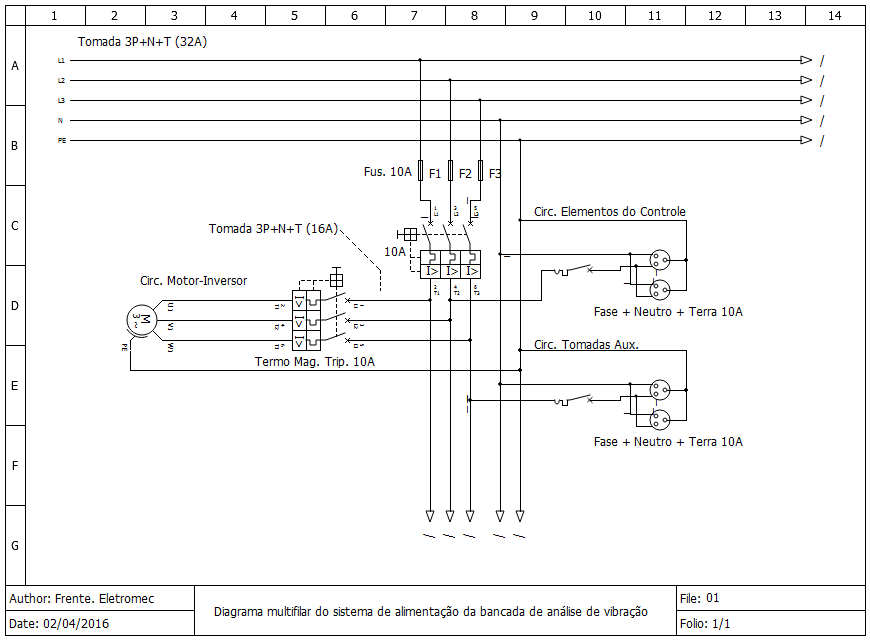
\includegraphics[keepaspectratio=true,scale=0.6]{figuras/Diagrama_Instalacao.png}
% 	\caption{Diagrama de Instalações e Sistema de Segurança}
%     \label{Diagrama de Instalações}
% \end{figure}